\documentclass[runningheads]{llncs}
\usepackage{fullpage}
\usepackage{graphicx} % for including images
\usepackage[T1]{fontenc}
\usepackage{subcaption}

\begin{document}
\title{Enhancing Urban Building Simulations in HiDALGO2 through CI/CD Innovations}
\author{Vincent Chabannes \inst{1}\orcidID{0000-1111-2222-3333} \and
Javier Cladellas \inst{1}\orcidID{} \and 
Abdoulaye Diallo \inst{1}\orcidID{} \and
Maryam Maslek \inst{1}\orcidID{} \and
Philippe Pinçon \inst{1}\orcidID{} \and
Christophe Prud'homme\inst{1}\orcidID{0000-0003-2287-2961}}
\institute{Cemosis, IRMA UMR 7501, University of Strasbourg, CNRS\\ 
\email{\{vincent.chabannes,christophe.prudhomme\}@cemosis.fr}}
\authorrunning{V. Chabannes and C. Prud'homme}


\maketitle

\begin{abstract}
The building sector in the European Union significantly impacts energy consumption and greenhouse gas emissions. The EU's Horizon 2050 initiative sets ambitious goals to reduce these impacts through enhanced building renovation rates. The HiDALGO2 project supports this initiative by developing high-performance computing solutions, specifically through the Urban Building pilot application, which utilizes advanced CI/CD methodologies to streamline simulation and deployment across various computational platforms.
\keywords{HPC, Urban building, City Energy Simulation.}

\end{abstract}

\section{Introduction}
The building sector accounts for approximately 40\% of final energy consumption and 36\% of greenhouse gas emissions within the European Union. In response, the EU has established ambitious targets under the Horizon 2050 framework to double energy renovation rates over the next decade, highlighting the need for innovative solutions to drive these initiatives forward. The HiDALGO2 project, with its focus on high-performance computing and advanced simulations, is at the forefront of tackling this challenge, particularly through its Urban Building pilot application.

The Urban Building pilot in HiDALGO2 aims to leverage high-performance computing to enhance urban simulations for better energy management and air quality assessment. This section outlines the specific objectives and expected impacts of the project.

Advanced simulation tools are employed to predict energy consumption, thermal comfort, and indoor air quality across both the building and urban scales. These simulations support detailed analysis at the individual building level and extend to broader urban environments, influencing urban planning and policy-making.

Integrating building simulations with urban air pollution models enables the project to assess the environmental impact of building stocks comprehensively. This integration improves the predictive accuracy of the simulations by incorporating real-time data such as wind speed and solar radiation, enhancing the models' responsiveness to environmental conditions.

Implementing these objectives will facilitate more informed urban planning decisions, support policy development for energy efficiency, and contribute to reducing urban greenhouse gas emissions. The project also focuses on enhancing the interaction between different environmental models to provide a holistic view of urban ecosystems.

\section{Overview of Urban Building Modeling and Simulation}

We now provide an overview of the geometrical and physical modeling and simulation components of the Urban building application.

\subsection{Geometry Reconstruction of the Urban Model}

The geometric reconstruction of urban environments within the HiDALGO2 project involves a sophisticated approach to creating multi-fidelity representations of buildings, terrain, vegetation, roads, and other urban elements. This section outlines the methodologies employed and the various levels of detail (LOD) used in the models.

The primary challenge lies in accurately representing the complex urban landscape to support various simulations. A tiled web map approach is adopted, which allows for distributed data management and adapts the Level of Definition (LOD) based on specific needs. However, this approach requires the careful integration of tiles to ensure seamless representation.

We describe our definition of Levels of Detail for Buildings
\begin{itemize}
    \item \textbf{LOD-0:} The simplest form, representing buildings as oriented bounding boxes. This level is typically used for large-scale preliminary analyses and quick visual assessments.
    \item \textbf{LOD-1:} Buildings are represented as polygonal extrusions, with added roof structures to improve the visual accuracy and utility in simulations that do not require detailed internal features.
    \item \textbf{LOD-2:} At this level, buildings are detailed using Industry Foundation Classes (IFC) standards, supporting detailed thermal and structural analyses. This includes detailed geometries for each entity of the building, often using complex surface models like B-REP, swept solids, or CSG techniques.
\end{itemize}


In the figure~\ref{fig:buildings}, we illustrate the different levels of details.

\begin{figure}[htbp]
\centering
\begin{subfigure}{.4\textwidth}
  \centering
  \includegraphics[width=\linewidth]{images/buildings-lod0.png}
  \caption{LOD-0}
  \label{fig:sub1}
\end{subfigure}%
\begin{subfigure}{.4\textwidth}
  \centering
  \includegraphics[width=\linewidth]{images/buildings-lod1.png}
  \caption{LOD-1}
  \label{fig:sub2}
\end{subfigure}
\begin{subfigure}{.4\textwidth}
  \centering
  \includegraphics[width=\linewidth]{images/buildings-lod2.png}
  \caption{LOD-2}
  \label{fig:sub3}
\end{subfigure}%
\begin{subfigure}{.4\textwidth}
  \centering
  \includegraphics[width=\linewidth]{images/buildings-lod2-zoom.png}
  \caption{LOD-2 with a zoom}
  \label{fig:sub4}
\end{subfigure}
\caption{}
\label{fig:buildings}
\end{figure}


Building meshes are generated from metadata fetched from web services like OpenStreetMap, which provides multi-polygons with holes, representing the complex urban fabric. For \textbf{LOD-0 and LOD-1}, buildings are modeled from 2D footprints extruded to form three-dimensional volumes. These volumes are then combined or subtracted to represent the district or the entire city, applying union operations on buildings that touch or intersect. In \textbf{LOD-2}, the focus shifts to creating conformal and watertight meshes that are suitable for detailed simulation tasks. These meshes are generated from Building Information Modeling (BIM) data in IFC format, enabling a detailed representation of each building component.

In the figure~\ref{fig:city-strasbourg}, we display an illustration of the center of the city of Strasbourg with LOD-0~\ref{fig:city-strasbourg-lod0} and LOD-1\ref{fig:city-strasbourg-lod1} representations.

\subsubsection{Terrain Modeling}
The terrain modeling process utilizes elevation data extracted from raster images. The initial step involves creating a uniform mesh based on the size of the raster image. Following this, the elevation at each node is evaluated. Subsequently, isolines for elevation are computed, and mesh adaptation techniques are applied to reduce mesh density where feasible. Finally, each tile is glued together to ensure the continuity of the terrain mesh.

\subsubsection{Integration of Terrain and Building Meshes}
This process involves creating a conforming mesh that includes both the terrain and the buildings, ensuring that buildings on slopes are accurately modeled by adapting their height and embedding them into the terrain mesh. The figure~\ref{fig:city-grenoble-terrain} illustrates this aspect.

\subsubsection{Visual Representation}
Advanced rendering techniques are employed to visualize the multi-fidelity urban models, supporting both detailed analysis and general urban planning discussions. These visualizations are crucial for assessing the impact of urban changes and for stakeholder engagement.

This approach enhances the accuracy, utility, and scalability of urban models, making them vital for comprehensive urban analysis and planning in the HiDALGO2 project.

\begin{figure}[htbp]
\centering
\begin{subfigure}{.4\textwidth}
  \centering
  \includegraphics[width=\linewidth]{images/city-strasbourg-lod-0.png}
  \caption{LOD-0}
  \label{fig:city-strasbourg-lod0}
\end{subfigure}%
\begin{subfigure}{.4\textwidth}
  \centering
  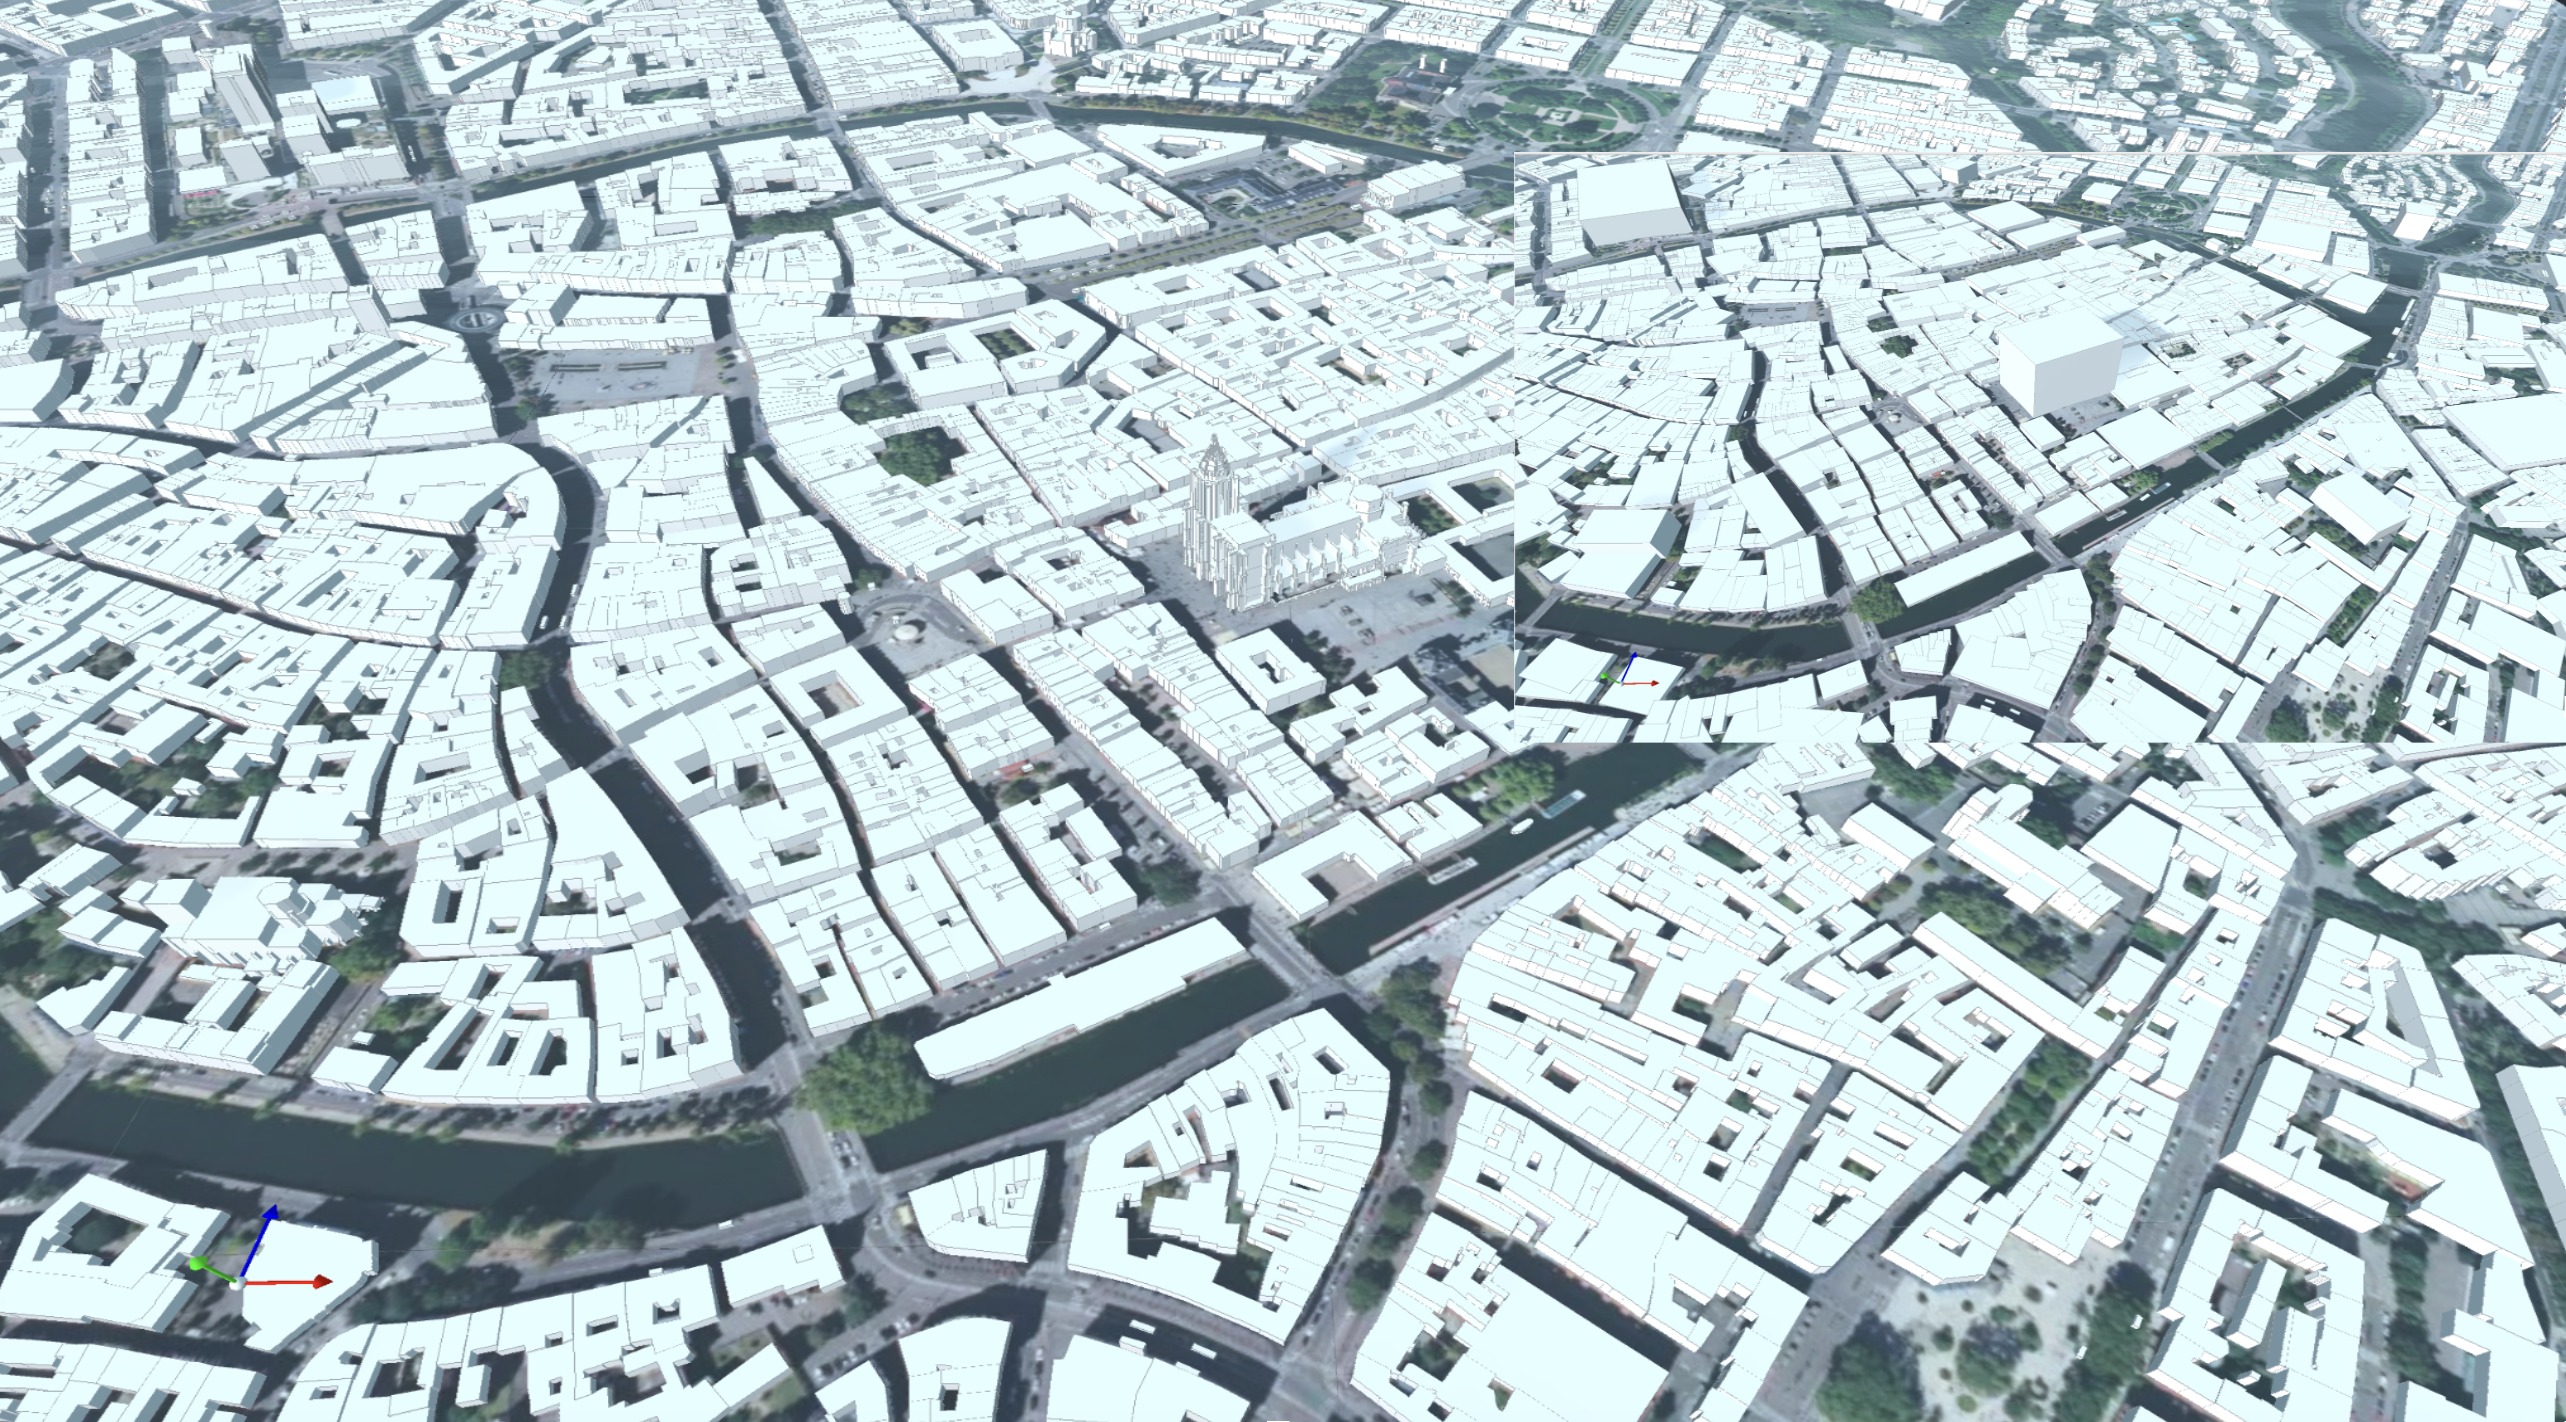
\includegraphics[width=\linewidth]{images/city-strasbourg-lod-1.png}
  \caption{LOD-1}
  \label{fig:city-strasbourg-lod1}
\end{subfigure}
\begin{subfigure}{.4\textwidth}
  \centering
  \includegraphics[width=\linewidth]{images/city-grenoble-terrain.png}
  \caption{LOD-1 terrain}
  \label{fig:city-grenoble-terrain}
\end{subfigure}
\caption{}
\label{fig:city-strasbourg}
\end{figure}

\subsubsection{Computational Tools for Building Meshes}

In the urban modeling process, particularly in the generation of building meshes, the Computational Geometry Algorithms Library (CGAL) plays a pivotal role. CGAL is renowned for its robust and efficient algorithms, which are crucial for handling complex geometric data and generating high-quality meshes from them.

\paragraph{Current Mesh Generation Strategy}
The current strategy for mesh generation employs multi-threading (MT) to handle various stages of the mesh construction process. Initially, the tiles to be used are determined based on the specified location, a task performed sequentially. Following this, GIS data, including buildings and elevation information, is downloaded in parallel. Next, polygons are repaired to ensure they are suitable for mesh generation, with this process executed in parallel using MT. The terrain mesh is then generated in parallel, employing CGAL's algorithms to ensure precision and efficiency. Union operations at tile junctions are performed to ensure continuity, a step that is currently sequential. Finally, building meshes are generated using a parallel MT approach, leveraging CGAL for its advanced mesh generation capabilities.

\paragraph{Advancing Towards Full Parallelism}
The next steps in enhancing the mesh generation process involve moving towards a fully parallel approach using both Multi-threading (MT) and Message Passing Interface (MPI). The goal is to scale the process up to handle entire cities or larger urban areas. This scale-up involves utilizing MPI to manage distributed computing resources effectively. To achieve this, partitions of tiles with overlapping areas are created to ensure complete and accurate building descriptions without the need for extensive MPI communication. Furthermore, each process uses an MT strategy to generate meshes independently, with overlapping zones allowing for the creation of complete building structures.

\subsubsection{Partitioning Strategies Depending on Simulation Use Cases}
Different partitioning strategies are employed depending on the specific requirements of the simulation use cases. For simple scenarios where buildings do not interact with their environment, a basic listing and weighting strategy is sufficient, known as Test Case 0. In Test Case 1, where buildings interact with environmental elements, a more complex partitioning strategy is necessary that considers both the buildings and their immediate non-building surroundings. For full interaction models, as in Test Case 2, the partitioning strategy starts with the buildings and extends to the entire urban mesh, ensuring that all elements are considered to minimize communication overhead. Looking towards scenarios with extreme partitioning needs, Test Case 3 employs a multigrid approach, defining coarse and fine meshes to efficiently manage computational resources. This multi-fidelity approach not only enhances the accuracy and applicability of urban models in simulations but also ensures scalability across different computational platforms, making it a cornerstone of urban analysis in the HiDALGO2 project.

The figure~\ref{fig:partitioning} illustrate the different strategies discussed previously and present a reconstruction of New York with 10km square reconstruction with hundreds of thousands of buildings which requires the large scale approach discussed but not yet implemented nor tested.
\begin{figure}[htbp]
\centering
\begin{subfigure}{.4\textwidth}
  \centering
  \includegraphics[width=\linewidth]{images/city-strasbourg-lod0-parts.png}
  \caption{LOD-0}
  \label{fig:city-strasbourg-lod0-parts}
\end{subfigure}%
\begin{subfigure}{.4\textwidth}
  \centering
  \includegraphics[width=\linewidth]{images/city-strasbourg-lod1-parts.png}
  \caption{LOD-1}
  \label{fig:city-strasbourg-lod1-parts}
\end{subfigure}
\begin{subfigure}{.4\textwidth}
  \centering
  \includegraphics[width=\linewidth]{images/city-newyork-largescale.png}
  \caption{LOD-1 Large scale}
  \label{fig:city-ny-largescale}
\end{subfigure}
\caption{}
\label{fig:partitioning}
\end{figure}

\subsubsection{Conclusion on mesh construction}
Our strategy not only aims to improve the efficiency and scalability of the mesh generation process but also enhances the fidelity and accuracy of the urban models used in simulations.

\subsection{Modeling and simulations}

We now turn to describing the physical modeling of  city energy simulation.
To do this we build on two main tools: Feel++ and Modelica. 

\subsubsection{Feel++ Toolchain}

Feel++ is a comprehensive framework designed to tackle problems based on Ordinary Differential Equations (ODEs) and Partial Differential Equations (PDEs). Utilizing modern C++ (C++17 and C++20) standards coupled with a Python layer through Pybind11, Feel++ enables seamless parallelism and is equipped with default communicators that simplify the handling of complex computational tasks. The framework's versatility is evident in its deployment across various platforms, which includes both research and educational environments, as well as cloud services tailored for high-performance computing needs.

Key features of the Feel++ framework include:
\begin{itemize}
    \item An extensive range of numerical methods to solve PDEs such as continuous Galerkin (cG), discontinuous Galerkin (dG), hybrid discontinuous Galerkin (hdG), and reduced basis methods (rb/mor).
    \item Domain Specific Language (DSL) for Galerkin methods which enhances the ease of implementing and experimenting with new numerical methods.
    \item The de Rham complex provides a comprehensive toolkit for constructing finite element spaces of arbitrary order.
    \item Automatic differentiation and symbolic integration bridge the gap between mathematical expressions and their implementation.
    \item The framework supports a diverse array of applications from fluid dynamics, structural mechanics, to heat transfer and electrostatics, demonstrating its flexibility and broad applicability.
    \item Integration with SpeCxx for task-based parallel execution, improving performance and scalability on modern computational architectures.
\end{itemize}

\paragraph{Simulation Tools and Applications}
Feel++ comes equipped with a variety of toolboxes tailored for specific application domains, offering pre-built scenarios for fluid dynamics, solid mechanics, and electromagnetism, among others. These toolboxes are designed to provide robust and efficient solutions, leveraging the capabilities of Feel++ to address complex multi-physics problems in real-world scenarios.

Documentation and further details can be accessed through [Feel++ Toolboxes Documentation](https://docs.feelpp.org/toolboxes/latest/).

This powerful toolchain is essential for the Urban Building pilot of the HiDALGO

\subsubsection{Computing Shading Masks and View Factors with Feel++}

In urban building energy simulations, the computation of shading masks and view factors is crucial for accurately modeling the impact of solar radiation on building surfaces. Shading masks quantify the percentage of blocked solar radiation for each building surface (including walls and roofs) depending on the direction of the sun. This is influenced by nearby structures such as other buildings, vegetation, and urban furniture. The view factors describe the fraction of radiation that leaves one surface and strikes another, which are essential for calculating radiative heat exchanges between building surfaces.

\paragraph{Numerical Methods and Challenges}
Both shading masks and view factors are computed using Monte Carlo and ray tracing techniques, which allow for handling complex geometries with various obstructions. Despite being purely geometric quantities, these calculations face significant challenges such as:
\begin{itemize}
    \item Efficient computation of integrals for view factors, especially when considering specular surfaces that require multiple ray bounces.
    \item Managing large-scale mesh computations and data storage, particularly when detailed urban environments are modeled.
\end{itemize}

\paragraph{Implementation in Feel++}
Feel++ facilitates these computations through its robust numerical methods optimized for high performance and parallel execution. For each face of a building, Feel++ computes solar masks using a Monte Carlo approach for various sun positions, ensuring efficient and scalable processing across multiple CPU cores. This enables the integration of dynamic solar shading effects into the simulation of building energy performance, providing a more accurate representation of real-world conditions.

\begin{figure}[htbp]
\centering
\begin{subfigure}{.4\textwidth}
  \centering
  \includegraphics[width=\linewidth]{images/solar-masks-east-facing.png}
  \caption{LOD-0}
  \label{fig:sm-building-east}
\end{subfigure}%
\begin{subfigure}{.4\textwidth}
  \centering
  \includegraphics[width=\linewidth]{images/solar-masks-whole-building.png}
  \caption{LOD-1}
  \label{fig:sm-whole-building}
\end{subfigure}
\begin{subfigure}{.4\textwidth}
  \centering
  \includegraphics[width=\linewidth]{images/solar-masks-strasbourg.png}
  \caption{LOD-1 Large scale}
  \label{fig:sm-strasbourg}
\end{subfigure}
\begin{subfigure}{.4\textwidth}
  \centering
  \includegraphics[width=\linewidth]{images/view-factors-benchmark.png}
  \caption{Heat transfer benchmark in 2D including view factors}
  \label{fig:view-factor}
\end{subfigure}
\caption{Solar masks and view factors computations}
\label{fig:solar-masks-vf}
\end{figure}

In the figure~\ref{fig:solar-masks-vf}, we illustrate \textit{(i)} the solar masks of building face oriented eastwise for a discretization of the sun position in the panel~\ref{fig:sm-building-east}, \textit{(ii)} the solar masks for an entire building for discretization of the sun position in the panel~\ref{fig:sm-whole-building}, \textit{(iii)} a visualization of the solar mask early morning of the city center of Strasbourg in panel~\ref{fig:sm-strasbourg} and \textit{(iv)} an image of a standard benchmark for the computation of view-factors and solving the heat transfer problems between three building blocks in 2D subsequently in panel~\ref{fig:view-factor}.

\subsubsection{Heat Transfer Modeling with Feel++ and Modelica}
In the Urban Building Energy Model (UBEM), heat transfer analysis is a crucial component for predicting energy consumption, internal air temperature variations, and overall building energy performance. This analysis is facilitated by a combination of Feel++ and Modelica, which together enable detailed simulations of heat dynamics within urban buildings.

\paragraph{Modelica for Multizone Heat Transfer}
Modelica offers extensive capabilities for multizone building energy simulations, utilizing models that range from simple (LOD-0) to more complex (LOD-1) representations. The multizone approach in Modelica is particularly useful for modular and scalable simulations, where each zone of the building can be modeled with different fidelity based on the simulation requirements. This method leverages the generation of Functional Mock-up Units (FMUs) which integrate seamlessly into larger C/C++ applications, providing a robust framework for handling complex simulations involving multiple interacting systems.

\paragraph{Finite Element Analysis with Feel++}
Complementing Modelica's capabilities, Feel++ provides robust tools for finite element analysis, particularly in handling the detailed aspects of heat transfer within urban environments. It uses advanced numerical methods like reduced basis methods for rapid scenario testing and parallel-in-time algorithms for efficient simulations. This is particularly important for assessing the impact of solar radiation and external shading, which are modeled using both geometric and dynamic shading masks derived from solar paths.

\paragraph{Integrated Approach}
The integration of Feel++ and Modelica is exemplified in their use of shading masks and view factors, critical for accurate solar heat gain calculations. These masks are computed using Monte Carlo simulations and ray tracing methods to assess the percentage of solar radiation impacting various building surfaces. This data feeds into the Modelica simulations, enhancing the accuracy of the thermal load predictions.

\paragraph{Challenges and Solutions}
One of the main challenges in urban building simulation is managing the computational load, which is addressed through hybrid computing strategies that leverage both CPUs and GPUs. This approach ensures that large-scale simulations, necessary for city-wide energy analysis, remain feasible and efficient. Additionally, the mesh partitioning techniques discussed earlier are employed to optimize the data handling and processing times, further integrating the spatial data management with the thermal modeling processes.

By utilizing the combined strengths of Feel++ for detailed finite element analysis and Modelica for system-level energy simulation, the UBEM framework achieves a comprehensive tool capable of addressing the complex dynamics of urban heat transfer and energy management.

\section{The Role of CI/CD in Urban Building Simulations}
Continuous Integration (CI) and Continuous Deployment (CD) are pivotal in the development and operation of the Urban Building pilot. These practices enable efficient management of complex simulation software, ensuring seamless integration and deployment across various computational infrastructures.

\subsection{Continuous Integration: Ensuring Code Quality and Reliability}
CI practices in HiDALGO2 handle complex dependencies and computational requirements specific to urban building simulations. Key features include automated testing, code quality checks, and automated builds, ensuring that the software remains robust and maintainable.

\subsection{Continuous Deployment: Streamlining Software Delivery}
CD practices are tailored to manage deployment complexities across different HPC environments using containerization through Apptainer. This approach facilitates consistent, reproducible deployments, optimizing performance and resource utilization.


\section{Current Urban Building Workflow}

\begin{figure}
    \centering
    \includegraphics[width=.9\textwidth]{images/kub-workflow.pdf}
    \caption{Current Urban Building Workflow}
    \label{fig:ub_workflow}
\end{figure}

The Urban Building workflow integrates various data sources and computational tools to simulate and analyze urban building energy and its impact on urban environments effectively. The following subsections detail each component of the workflow as depicted in the provided diagram.

\subsection{Data Acquisition and Preparation}
\begin{itemize}
    \item \textbf{Location Data:} Initial GIS data related to the specific location.
    \item \textbf{Weather Data Integration:} Incorporation of both regulatory and open-source weather data through the MeteoGrid system, which is then transformed into a usable format for simulations.
\end{itemize}

\subsection{Data Processing}
\begin{itemize}
    \item \textbf{Partitioning:} The GIS data and 3D mesh data are partitioned for scalable processing.
    \item \textbf{UBEM Generator:} Converts GIS data into Modelica and FEEL++ compatible formats for simulation.
\end{itemize}

\subsection{Simulation and Analysis}
\begin{itemize}
    \item \textbf{Urban Building Energy Model (UBEM):} Uses converted data to simulate energy consumption and indoor environmental quality.
    \item \textbf{Radiative Heat Transfer:} Calculation of heat transfer effects due to radiation, enhancing the accuracy of the energy models.
    \item \textbf{View Factors and Shading Masks:} Computes how buildings affect each other's exposure to natural light and heat, influencing the urban heat island effect and building energy needs.
\end{itemize}

\subsection{Coupling with Urban Air Pollution Model}
\begin{itemize}
    \item \textbf{Integration with UAP:} The building simulation outputs are fed into the Urban Air Pollution (UAP) simulator to assess the impact of building emissions on urban air quality.
    \item \textbf{Feedback Loop:} Intermediate outputs from the UAP simulator are utilized to refine building simulation scenarios.
\end{itemize}

\subsection{Final Output and Urban Scale Energy Analysis}
\begin{itemize}
    \item \textbf{UBEM Simulator:} Generates final outputs that summarize the overall energy consumption and environmental impact of buildings at an urban scale.
    \item \textbf{Comprehensive Urban Scale Analysis:} The final integration step where data from both the building energy models and air quality models are combined to provide a holistic view of urban environmental quality.
\end{itemize}

This workflow is critical for accurately simulating and understanding the complex interdependencies between urban building energy usage and urban air quality, supporting the broader objectives of the HiDALGO2 project to improve urban living conditions and sustainability.


\section{Software Stack and CI/CD Framework for the Urban Building Pilot}
The Urban Building pilot within the HiDALGO2 project leverages a sophisticated software stack centered around the Feel++ framework. This section details the components of the software stack and explains how the CI/CD framework facilitates efficient development and deployment.

\subsection{Feel++ Framework Capabilities}
Feel++ is a versatile framework designed for solving complex partial differential equations (PDEs) using high-performance computing (HPC). The capabilities of Feel++ are critical to the simulation tasks performed in the Urban Building pilot.

\begin{itemize}
    \item \textbf{Modular Software Stack:} Feel++ supports a range of functionalities essential for computational fluid dynamics (CFD), computational solid mechanics (CSM), and thermal simulations. Its software stack includes:
    \begin{itemize}
        \item MPI C++17/20 and Boost for parallel computing.
        \item PETSc for scalable and efficient numerical solutions.
        \item Python bindings for scripting and automation.
        \item Modelica integration for multidomain physical modeling and simulation.
    \end{itemize}

    \item \textbf{Simulation Capabilities:}
    \begin{itemize}
        \item Advanced solvers for fluid dynamics, heat transfer, and electromagnetic simulations.
        \item Support for reduced order methods, enhancing computational efficiency.
        \item Integration with data assimilation, machine learning, and uncertainty quantification to improve prediction accuracy and robustness.
    \end{itemize}
\end{itemize}

\subsection{CI/CD Using GitHub Actions and Docker}
The development and deployment of the Urban Building pilot are streamlined through a CI/CD pipeline that utilizes GitHub Actions and Docker. This setup ensures that the software development lifecycle is robust, with continuous integration and deployment enhancing productivity and reliability.

\begin{itemize}
    \item \textbf{GitHub Actions:} Automates workflows to compile, test, and validate code changes in real-time, facilitating rapid development cycles and ensuring code quality.
    \item \textbf{Docker:} Provides a containerized environment where Feel++ and its dependencies are encapsulated, ensuring consistent operations across different computing environments. Docker images are specifically tailored for various systems, accommodating a wide range of deployment scenarios.
\end{itemize}

% \subsection{Integration with Urban Air Pollution Models}
% As part of the CI/CD pipeline, the integration testing includes coupling with % urban air pollution models to evaluate the impact of simulated building parameters % on urban air quality. This ensures that the software stack not only performs as % expected in isolated tests but also behaves correctly in integrated urban % simulation environments.
% 

\section{CI/CD DevOps for Feel++}
The Continuous Integration and Continuous Deployment (CI/CD) pipeline is central to the development and maintenance of the Feel++ framework, ensuring that updates and enhancements are efficiently integrated and deployed across all projects utilizing Feel++. Below we outline the structured approach taken using GitHub Actions, Docker, and Apptainer.

\subsection{Feel++ Environment Setup}
Feel++ utilizes a robust environment setup that is continuously integrated and uploaded to GitHub Container Registry (ghcr.io). The environment includes configurations for multiple operating systems and computational backends:
\begin{itemize}
    \item Continuous Integration (CI) environments for Ubuntu 22.04, Ubuntu 20.04, Ubuntu 24.04, and Debian 12.
    \item Scheduled Integration (SCI) environments include Spack-based configurations for MPI and other computational libraries.
\end{itemize}

\subsection{Pipeline Trigger Mechanisms}
The CI/CD pipelines for Feel++ are triggered through various mechanisms to ensure responsiveness and up-to-date compatibility:
\begin{itemize}
    \item \textbf{Pull Requests and Merges:} Triggers the CI to ensure that new code integrations meet all tests and standards.
    \item \textbf{Graphical User Interface (GUI):} Allows developers to manually trigger pipelines through a GUI, facilitating quick deployments or tests.
    \item \textbf{Scheduled Runs:} Ensures regular updates and maintenance checks are performed, even during periods of low manual activity.
\end{itemize}

\subsection{Docker and Apptainer Workflow}
\begin{itemize}
    \item \textbf{Docker Images:} All Docker images are tailored for specific system requirements and are uploaded to ghcr.io. These images are then utilized to ensure consistent environments across various deployment scenarios.
    \item \textbf{Apptainer Images:} Apptainer (formerly Singularity) provides a secure way to handle containers. Images created for Apptainer ensure that Feel++ can be deployed in a secure and reproducible manner across HPC environments without requiring root privileges.
\end{itemize}



\subsection{Utilization by Projects}
\begin{itemize}
    \item Both Docker and Apptainer images are extensively used by projects built upon the Feel++ framework. These projects benefit from the robust, tested, and secure environments that Feel++ CI/CD practices ensure.
\end{itemize}

\section{HPC Operations (HPC-Ops)}
Innovative HPC-Ops practices are integral to the deployment and benchmarking processes of the Feel++ framework, enabling it to perform consistently across diverse high-performance computing (HPC) systems. This section details the strategies and tools used for large-scale computational benchmarks and reproducibility assurance.

\subsection{Benchmarking and Reproducibility}
Upon successful updates or integrations, large-scale benchmarking is triggered to evaluate the performance and scalability of the Feel++ applications. These benchmarks are crucial for:
\begin{itemize}
    \item Validating the computational correctness and efficiency across platform variations.
    \item Ensuring that performance optimizations are effective and do not introduce errors.
\end{itemize}

\subsection{Integration with HPC Systems}
\begin{itemize}
    \item \textbf{Apptainer Images:} Central to the HPC-Ops strategy, Apptainer (formerly Singularity) images are used to encapsulate the computing environment, making it portable and reproducible across all HPC platforms. These images are maintained and updated on GitHub Container Registry (ghcr.io).
    \item \textbf{HPC Systems:} The workflow is designed to integrate with several EuroHPC systems such as LUMI, Karolina, Meluxina, and Discoverer, as well as other significant HPC infrastructures including local systems like Gaya and global platforms such as PSNC/Eagle.
\end{itemize}

\subsection{Automation Tools}
\begin{itemize}
    \item \textbf{Reframe:} Used for defining and managing systematic benchmarks that are reproducible across various HPC environments.
    \item \textbf{GitHub Actions:} Automates the CI/CD pipeline, ensuring that any changes to the codebase are consistently and reliably deployed across all environments.
    \item \textbf{SLURM:} A key component in scheduling and managing jobs on many of the integrated HPC systems, facilitating efficient resource management and job queueing.
\end{itemize}

\subsection{Challenges and Solutions}
Discussing the challenges encountered in integrating such a diverse array of systems and the innovative solutions developed, including:
\begin{itemize}
    \item Ensuring compatibility and performance across different HPC architectures.
    \item Automating the deployment and scaling of complex simulations in a secure and efficient manner.
\end{itemize}

\subsection{Conclusion}
The HPC-Ops framework developed for Feel++ represents a significant advancement in the field of computational sciences, driving forward the capabilities for large-scale scientific computations. It sets a benchmark for how modern software frameworks can integrate with advanced HPC infrastructures to enhance computational research and applications.

\section{Urban Building DevOps Framework}

\subsection{Source Control and Management}
GitHub serves as the central repository hosting the source code, with robust version control to manage contributions and revisions effectively.

\subsection{Continuous Integration and Deployment (CI/CD)}
\begin{itemize}
    \item \textbf{Feel++ Environment Setup}: Leveraging Docker and Apptainer containers ensures a consistent and reproducible environment across different systems. Docker images are tailored to support various operating systems and configurations, which are regularly updated and pushed to GitHub Container Registry (ghcr.io).
    \item \textbf{Automated Testing and Deployment}:
    \begin{itemize}
        \item GitHub Actions automates workflows for testing, building, and deploying applications. This includes automatic updates for documentation hosted on GitHub Pages.
        \item Integration with GitHub ensures that code changes trigger automated workflows that build and test the software across multiple platforms.
    \end{itemize}
\end{itemize}

\subsection{Packaging}
The software is packaged into Wheel for Python libraries and DEB packages for Debian/Ubuntu systems. These packages facilitate easy distribution and installation of the software. Spack, a flexible package manager, is used for managing the installations of software on HPC systems, ensuring that dependencies are handled correctly across different environments.

\subsection{Deployment on HPC Systems}
Utilizing Apptainer (formerly Singularity) containers enhances portability and security, allowing the Urban Building simulations to be deployed seamlessly on various HPC systems including local clusters like Gaya and EuroHPC systems such as LUMI, Karolina, Meluxina, and Discoverer. The use of SLURM for job scheduling on these HPC systems ensures efficient management of computational resources.

\subsection{Documentation and Training}
Documentation is automatically generated and updated with each code push to the master branch, ensuring that all features and changes are well-documented. The documentation includes comprehensive guides on installation, configuration, and usage, along with API documentation generated directly from the source code.

\subsection{Benchmarking and Quality Assurance}
Continuous benchmarking is integrated into the CI/CD pipeline, triggering large-scale benchmark tests upon successful preliminary tests. This ensures that the software performs optimally across all supported platforms before any releases. Quality assurance practices include code reviews, unit testing, and integration testing, all automated through GitHub Actions.

By leveraging these DevOps practices, the Urban Building pilot ensures that it remains robust, scalable, and adaptable to new HPC technologies and architectures, ultimately supporting the HiDALGO2 project's goals of advancing urban simulation technologies at a global scale.


\section{Urban Building HPC Operations}

The Urban Building High-Performance Computing (HPC) Operations outline a sophisticated workflow that integrates continuous integration and deployment (CI/CD) with advanced benchmarking strategies. These operations are crucial for ensuring the performance, scalability, and reliability of the Urban Building simulations on various HPC systems.

\subsection{HPC Benchmarking CI/CD}
The benchmarking CI/CD pipeline is triggered upon successful completion of the standard CI/CD processes, which include automated testing and validation of the software. New Apptainer containers are created and made available, facilitating deployment on diverse computational resources.

\begin{itemize}
    \item \textbf{Automated Testing:} Once new changes are integrated and the standard CI/CD pipeline succeeds, larger scale tests are automatically initiated on a designated HPC node with significant computational resources, for example, 128 cores.
    \item \textbf{Manual and Scheduled Testing:} For extensive validation, tests can also be manually triggered or scheduled to run at predefined intervals. This flexibility allows for comprehensive performance assessments under varying loads and configurations.
\end{itemize}

\subsection{Use of Reframe}
Reframe is employed as the regression testing framework, essential for verifying the stability and performance regressions of the software across updates. It enables:
\begin{itemize}
    \item Systematic execution of test suites across different HPC systems.
    \item Collection and analysis of performance data to monitor software behavior and performance trends over time.
\end{itemize}

\subsection{Integration with HPC Systems}
\begin{itemize}
    \item \textbf{EuroHPC Integration:} The Urban Building pilot is integrated with several EuroHPC systems like LUMI, Karolina, Meluxina, and Discoverer, enhancing the capability to perform simulations at an unprecedented scale.
    \item \textbf{Local and International HPC Systems:} The framework also supports deployment on local HPC systems (e.g., Gaya) and international platforms like PSNC's Eagle, ensuring wide accessibility and usability of the software.
\end{itemize}

\subsection{Monitoring and Reporting}
All performance results are automatically captured and uploaded to the HiDALGO2 portal. This ensures that:
\begin{itemize}
    \item Stakeholders have real-time access to performance reports.
    \item Decision-makers can review comprehensive data to guide further optimization and development efforts.
\end{itemize}

\subsection{Deployment and Scalability}
\begin{itemize}
    \item \textbf{Containerized Deployment:} Utilizing Docker and Apptainer containers ensures that the Urban Building application is portable and consistent across various computing environments.
    \item \textbf{Scalable Benchmarking:} The capability to scale tests according to the available hardware and project requirements is critical, allowing the team to simulate urban environments of varying complexities.
\end{itemize}

This comprehensive HPC operations framework underlines the commitment of the HiDALGO2 project to leveraging cutting-edge computational technologies to enhance urban simulation studies, ensuring high performance and accuracy of the Urban Building models.

\section{Conclusion}
The CI/CD practices in Feel++ not only enhance the development lifecycle of the framework itself but also ensure that all dependent projects maintain high standards of reliability, security, and performance. The integration of Docker and Apptainer into the workflow enables wide-ranging deployment scenarios from personal computing environments to high-performance computing clusters.

The integration of Feel++ within the HiDALGO2 project's Urban Building pilot through a sophisticated CI/CD framework supports the project's goal to enhance urban sustainability and air quality. The continuous development, testing, and deployment facilitated by this framework are vital for adapting to evolving urban challenges and computational needs.


\section{Conclusion}
CI/CD practices in HiDALGO2 are vital for advancing urban building simulations, supporting the EU's energy efficiency goals, and contributing to the reduction of greenhouse gas emissions in the urban sector.

\begin{credits}
\subsubsection{\ackname} Hidalgo2, Exa-MA, ITI Irmia++ 

% \subsubsection{\discintname}
% It is now necessary to declare any competing interests or to specifically
% state that the authors have no competing interests. Please place the
% statement with a bold run-in heading in small font size beneath the
% (optional) acknowledgments\footnote{If EquinOCS, our proceedings submission
% system, is used, then the disclaimer can be provided directly in the system.},
% for example: The authors have no competing interests to declare that are
% relevant to the content of this article. Or: Author A has received research
% grants from Company W. Author B has received a speaker honorarium from
% Company X and owns stock in Company Y. Author C is a member of committee Z.
\end{credits}

\bibliographystyle{splncs04}
\bibliography{mybib}

\end{document}